
\chapter{MPMICE} \label{Sec:MPMICE}

\section{Introduction}

MPMICE is a marriage of the multi-material ICE method, described in
Section~\ref{Sec:ICE} and MPM, described in Section~\ref{Sec:MPM}.
The equations of motion solved for both fluid and solid are essentially
the same, although the physical behavior of these two states of matter
differ, largely due to their constitutive relationships.  MPM is used
to track the evolution of solid materials in a Lagrangian frame of
reference, while fluids are evolved in the Eulerian frame.

\section{Theory - Algorithm Description}

At this time, the reader is directed to the manuscript by Guilkey,
Harman and Banerjee~\cite{fourthmit} for the theoretical and algorithmic
description of the method.

%\subsection{Uintah Specification}

%\subsubsection{ICE}

%\subsubsection{Basic Inputs}
%\subsubsection{Physical Constants}
%\subsubsection{Material Properties}
%\subsubsection{Equation of State}
%\subsubsection{Exchange Properties}
%\subsubsection{BoundaryConditions}
%\subsubsection{Solvers}


%\subsection{MPM}

%\subsubsection{Basic Inputs}
%\subsubsection{Physical Constants}
%\subsubsection{Material Properties}
%\subsubsection{Constitutive Models}
%\subsubsection{Contact}
%\subsubsection{BoundaryConditions}
%\subsubsection{Physical Boundary Conditions}

\section{Solid State Kinetic Models}

A generalized reaction model for solid state kinetics based on the
assumption that the temperature dependence of the rate can be separated
from the reaction model as embodied by the equation:

\begin{equation}
\frac{d\alpha}{dt}=k(T)f(\alpha)
\end{equation}

\noindent is implemented in Uintah and named \textbf{SolidReactionModel}.  To
use the \textbf{SolidReactionModel} one must specify both a temperature
dependent rate constant model and a rate model.  The model is a grid based
model, so should work with both MPM and ICE materials.  In the case where an MPM
material is used as the reactant or product, the thermodynamic quantities
that are interpolated to the grid are used to calculate reaction rates.   

Additional rate constant and rate models may be added by either subclassing \textbf{RateConstantModel}
or \textbf{RateModel}.  Examples of this can be found in the 
\textbf{src/CCA/Components/Models/SolidReactionModel}
directory. Two models currently exist for the rate constant $k(T)$, Arrhenius and
Modified Arrhenius.  These two models have the forms:

\begin{equation}
k(T)=Ae^{\frac{-E_a}{RT}}
\end{equation}

\noindent and:

\begin{equation}
k(T)=AT^be^{\frac{-Ea}{RT}}
\end{equation}

Various rate models of different classes exist for use.  These classes include
reaction-order models, diffusion models, geometrical contraction models and
nucleation models. The following table shows the various models available.  Models
were taken from \cite{ref:vyazovkinwight} and \cite{ref:khawamflanagan}.\newline\newline

\begin{tabular}{ |l | c | c |}
\hline
\textbf{Model} & $f(\alpha)$ & \textbf{Uintah 'type'} \\
\hline
\hline
\multicolumn{3}{|c|}{\textbf{Reaction-order Models}} \\
\hline
Nth Order & $(1-\alpha)^n$  & NthOrder \\
\hline
\multicolumn{3}{|c|}{\textbf{Diffusion Models}} \\
\hline
1-D Diffusion & $1/2\alpha$  & Diffusion \\
\hline
2-D Diffusion & $-1/ln(1-\alpha)$  & Diffusion \\
\hline
3-D Diffusion& $3/2(1-\alpha)^{2/3}(1-(1-\alpha)^{1/3})$  & Diffusion \\
\hline
4-D Diffusion& $3/2(1/\alpha^{1/3}-1)$  & Diffusion \\
\hline
\multicolumn{3}{|c|}{\textbf{Geometrical Contraction Models}} \\
\hline
Contracting Cylinder& $2\sqrt{1-\alpha}$  & ContractingCylinder \\
\hline
Contracting Sphere& $3(1-\alpha)^{2/3}$  & ContractingSphere \\
\hline
\multicolumn{3}{|c|}{\textbf{Nucleation Models}} \\
\hline
Power & $a\alpha^b$  & Power \\
\hline
Avarami-Erofe'ev & $a(1-\alpha)(-ln(1-\alpha))^b$  & AvaramiErofeev \\
\hline
\end{tabular} \newline\newline

The input file specification is as follows:

\begin{verbatim}
  <Models>
    <Model type="SolidReactionModel">
      <RateConstantModel type="type">
         ....
      </RateConstantModel>
      <RateModel type="type">
         ....
      </RateModel>
    </Model>
  <Models>
\end{verbatim}

\noindent Here, the type attribute for \textbf{RateConstantModel} should be either \textbf{Arrhenius} or \textbf{ModifiedArrhenius}
which both take an activation energy \textbf{Ea}, and frequency factor \textbf{A}.  In addition, the modified Arrhenius
model takes a temperature dependence exponent, \textbf{b}.

The specification of type attribute for \textbf{RateModel} should be one of those listed in the previous table.
The \textbf{NthOrder} model must have a positive integral value for the reaction order \textbf{n}. 
The \textbf{Diffusion} based models require a \textbf{dimension} value that should be 1, 2, 3 or 4 depending
on the dimensionality of the desired rate model.  Both geometric contraction models take no additional
input parameters. Both nucleation based models, \textbf{Power} and \textbf{AvaramiErofeev}, take both 
an \textbf{a} and a \textbf{b} input parameter. 

\section{HE Reaction Models}

Three models exist for reaction of high explosive materials.  Each
simulation using one of these models utilize MPMICE's material
interactions as its foundation.  The components work by taking several
material specific constants as well as a reactant and product material
from the model input section of the .ups file.  Following are brief
descriptions of each model, as well as their input parameters.

\subsection{Simple Burn} \label{Sec:SimpleBurn}

Simple Burn, as the name implies, is a simple model of combustion of HMX based on the rate equation:

\begin{equation}
\dot{m}=A P^{0.778}
\label{simburneqn}
\end{equation}

Where $\dot{m}$ is the mass flux, $P$ is the pressure and $n$ is the pressure dependence coefficient.  The pressure coefficient in Equation (\ref{simburneqn}) is that of HMX.  The models input section for a Simple Burn simulation takes the form: 

\begin{verbatim}
<Models>
  <Model type="Simple_Burn">
    <fromMaterial> reactant      </fromMaterial>
    <toMaterial>   product       </toMaterial>
    <Active>       true          </Active>
    <ThresholdTemp>       450.0  </ThresholdTemp>
    <ThresholdPressure> 50000.0  </ThresholdPressure>
    <Enthalpy>        2000000.0  </Enthalpy>
    <BurnCoeff>            75.3  </BurnCoeff>
    <refPressure>      101325.0  </refPressure>
  </Model>
</Models>
\end{verbatim}

The first two tags take names of materials previously defined in the input file, defining both reactant and product used by the model.  See Section \ref{sec:ICEmat_props} and \ref{Sec:mat_props} for in depth description for defining materials.  $<$Active$>$ is a debugging parameter that takes a boolean value indicating whether the model is on (i.e. the actual computations take place during the timestep).  True is the value to set for $<$Active$>$ in most situations.  Each of the other parameters take double values.  Threshold temperature and pressure tags define two criteria the cell must have in order to be flagged burning.  The reference pressure is used to scale the cell centered pressure as well as make it an unitless value.  The burn coefficient corresponds to $A$ in the rate equation.  Enthalpy is simply the enthalpy value for conversion of reactant to product.
\newpage
\subsection{Steady Burn} \label{Sec:SteadyBurn}

Steady Burn is a more accurate model than Simple Burn.  It is based on WSB model of combustion developed by Ward, Son and Brewster in \cite{ref:wardsonbrewster}.  WSB is based on a simplified two-step chemical model with an initial zero-order, thermally activated ($E_c > 0$), mildly exothermic, solid-to-gas reaction, modeled as a thermal decomposition of the solid:

\begin{equation}
A(solid)\rightarrow B(gas)
\end{equation}

Intermediate $B$, in the presence of any gas phase collision partner $M$, reacts in a highly exothermic fashion producing a flame.  This step is modelled as a second-order, gas phase, free radical chain reaction based on the assumption that $E_g = 0$:

\begin{equation}
B(gas)+M(gas)\rightarrow C(gas)+M(gas)
\end{equation}

As such, this second equation represents the reaction in the gas phase that causes heat convection back to the surface that activate the first reaction.  In Steady Burn, a solution is found by iteratively solving two equations: one for mass burning rate $\dot{m}$ and one for surface temperature $T_s$.  Mass flux is initially solved with an assumed value $T_s$ (in the model set to $850.0 K$) using WSB:

\begin{equation}
\dot{m}\left(T_s\right)=\sqrt{\frac{\displaystyle \kappa_c \rho_c A_c R T_s^2 \exp\left({\frac{\displaystyle -E_c}{\displaystyle R T_s}}\right)}{\displaystyle C_p E_c \left(T_s - T_0 - \frac{Q_c}{2 C_p}\right)}}
\label{WSB1}
\end{equation}

The solution to this equation is used to refine the surface temperature and vice-versus until a self-consistent solution for surface temperature and mass flux has been found.  The surface temperature equation takes the form:

\begin{equation}
T_s(\dot{m},P)=T_0 + \frac{\displaystyle Q_c}{\displaystyle C_p} + \frac{Q_g}{Cp\left(1+\frac{\displaystyle x_g\left(\dot{m},P\right)}{\displaystyle x_{cd}(\dot{m})}\right)}
\label{WSB2}
\end{equation}

$x_g$ in the third term of Equation (\ref{WSB2}) is the flame standoff distance, computed from:

\begin{equation}
x_g\left(\dot{m},P\right)=\frac{2 x_{cd}\left(\dot{m}\right)}{\displaystyle \sqrt{1 + D_a\left(\dot{m},P\right)} - 1}
\label{WSB3}
\end{equation}

where $x_{cd}$ and $D_a$ are the convective-diffusive length and Damkohler number, respectively:

\begin{equation}
x_{cd} \left(\dot{m}\right)=\frac{\kappa_g}{\displaystyle \dot{m} C_p}
\label{WSB4}
\end{equation}
\begin{equation}
D_a\left(\dot{m},P\right) = \frac{4 B_g M C_p P^2}{\displaystyle R^2 \kappa_g} x_{cd}\left(\dot{m}\right)^2
\label{WSB5}
\end{equation}

WSB model is valid as a 1D model, but needs extension to work in a 3D multimaterial CFD environment.  As such, Steady Burn is WSB extended with logic for ignition of energetic materials and computation of surface area for burning cells.  Ignition of a cell is based on three criteria: 
\begin{itemize}
  \item The cell must contain one particle of energetic solid
  \item The cell is near a surface of an energetic solid (e.g. ratio of minimum node-centered mass to maximum node-centered mass is less than 0.7)
  \item One neighboring cell must have at most two particles of energetic material
\end{itemize}
If a cell is ignited, the model will be applied and mass will be transferred from reactant material to product material.  Total mass burned is computed using mass flux $\dot{m}$, $\Delta t$ of the timestep and the calculated surface area, found using:

\begin{equation}
A=\frac{\delta x \delta y \delta z}{\displaystyle \delta x |g_x| + \delta y |g_y| + \delta z |g_z|}
\label{WSB6}
\end{equation} where $\delta x$, $\delta y$, and $\delta z$ are the dimensions of the cell and components of $\overrightarrow{g}$ are the normalized density gradients of the particle mass in a cell.  A more thorough examination of Steady Burn can be read about in \cite{ref:wighteddings}.

The following table describes the input parameters for Steady Burn.  The final column of the table indicates parameters for combustion of HMX.  

\begin{center}
\begin{tabular}{| l | c | p{4cm} | l |}
\hline
  \multicolumn{4}{|c|}{\textbf{Steady Burn Input Parameters}} \\
\hline
\hline
  \textbf{Tag} & \textbf{Type} & \textbf{Description} & \textbf{HMX Value} \\
\hline
  $<$fromMaterial$>$ & String & `Name' of reactant material (mass source) &  \\
\hline
  $<$toMaterial$>$ & String & `Name' of product material (mass sink) & \\
\hline
  $<$IdealGasConst$>$ & double & Ideal gas constant ($R$) & $8.314 J/(K\times mol)$ \\
\hline
  $<$PreExpCondPh$>$ & double & Condensed phase pre-exponential coefficient ($A_c$) & $1.637\times10^{15} s^{-1}$ \\
\hline
  $<$ActEnergyCondPh$>$ & double & Condensed phase activation energy ($E_c$) & $1.76\times10^5 J/mol$ \\
\hline
  $<$PreExpGasPh$>$ & double & Gas phase frequency factor ($B_g$) & $1.6\times10^{-3} m^3/(kg\times s\times K)$ \\
\hline
  $<$CondPhaseHeat$>$ & double & Condensed phase heat release per unit mass ($Q_c$) & $4.0\times10^5 J/kg$ \\
\hline
  $<$GasPhaseHeat$>$ & double & Gas phase heat release per unit mass ($Q_g$) & $3.018\times10^6 J/kg$ \\
\hline
  $<$HeatConductGasPh$>$ & double & Thermal conductivity of gas ($\kappa_g$) & $0.07 W/(m\times K)$ \\
\hline
  $<$HeatConductCondPh$>$ & double & Thermal conductivity of condensed phase ($\kappa_c$) & $0.02 W/(m\times K)$ \\
\hline
  $<$SpecificHeatBoth$>$ & double & Specific heat at constant pressure ($c_p$) & $1.4\times10^3 J/(kg\times K)$ \\
\hline
  $<$MoleWeightGasPh$>$ & double & Molecular weight of gas ($W$) & $3.42\times10^{-2} kg/mol$ \\
\hline
  $<$BoundaryParticles$>$ & int & Max \# of particles a cell can have and be burning & Resolution dependent \\
\hline
  $<$ThresholdPressure$>$ & double & Threshold pressure cell must have $\ge$ to burn mass & $50000 Pa$ \\
\hline
  $<$IgnitionTemp$>$ & double & Temperature cell must have $\ge$ to be burning & $550 K$ \\
\hline
\end{tabular}
\end{center}

\newpage
\subsection{Unsteady Burn} \label {Sec:UnsteadyBurn}

Unsteady Burn is a model developed at the University of Utah as an extension of Steady Burn to better represent mass burning rates when pressure at the burning surface fluctuates. A pressure-coupled response is accounted for in the model such that, qualitatively a pressure increase causes gas phase reaction rates to increase as well as move the gas phase reactions closer to the burning surface.  Increase of near surface gas phase reactions increases the rate of thermally activated solid state reactions, ultimately causing a higher steady burn rate.  Unsteady Burn more accurately models the transition from low pressure to high pressure than Steady Burn by taking into account the initially overshot burn rate at the time when the pressure increases, and the relaxation period to steady burn rate.  Similarly, Unsteady Burn models undershot pressures during pressure drops.  

The model is an extension of Steady Burn by partial decoupling of the gas phase and solid state Equations (\ref{WSB1}) and (\ref{WSB2}).  An expression for the temperature gradient of the solid:

\begin{equation}
  \beta = \left(T_s - T_0\right) \frac{m c_p}{\displaystyle\kappa_c}
  \label{WSB7}
\end{equation}

is reaarranged for $(T_s-T_0)$ and substituted in Equation (\ref{WSB1}) leading to the quadradic equation:

\begin{equation}
\dot{m}^2 - \frac{2 \beta \kappa_c}{Q_c} \dot{m} + \frac{2 A_c R T_s^2 \kappa_c \rho_c }{E_c Q_C} \exp\left({\frac{-E_c}{R T_s}}\right)=0
\label{WSB8}
\end{equation}

which allows independent tracking of temperature gradient $\beta$ and surface temperature $T_s$.  The gas phase response is computed using a runnning average of $T_s$ as it approaches the steady burning value.  A solid state response is obtained by computing a running average of $\beta$ as it approaches the steady burning value.  A slow relaxation time for $\beta$ and a fast relaxation time for $T_s$ models the overshoot or undershoot in burn rate.  Burning criteria for a cell is the same as Steady Burn.  For more information on Unsteady Burn see \cite{ref:wighteddings}.

The following table describes the input parameters for Unsteady Burn.

\begin{center}
\begin{tabular}{| l | c | p{7cm} |}
\hline  
  \multicolumn{3}{|c|}{\textbf{Unsteady Burn Input Parameters}} \\
\hline
\hline
  \textbf{Tag} & \textbf{Type} & \textbf{Description}\\
\hline
  $<$fromMaterial$>$ & String & `Name' of reactant material (mass source)\\
\hline
  $<$toMaterial$>$ & String & `Name' of product material (mass sink)\\
\hline
  $<$IdealGasConst$>$ & double & Ideal gas constant ($R$)\\
\hline
  $<$PreExpCondPh$>$ & double & Condensed phase pre-exponential coefficient ($A_c$) \\
\hline
  $<$ActEnergyCondPh$>$ & double & Condensed phase activation energy ($E_c$)\\
\hline
  $<$PreExpGasPh$>$ & double & Gas phase frequency factor ($B_g$)\\
\hline
  $<$CondPhaseHeat$>$ & double & Condensed phase heat release per unit mass ($Q_c$)\\
\hline
  $<$GasPhaseHeat$>$ & double & Gas phase heat release per unit mass ($Q_g$)\\
\hline
  $<$HeatConductGasPh$>$ & double & Thermal conductivity of gas ($\kappa_g$)\\
\hline
  $<$HeatConductCondPh$>$ & double & Thermal conductivity of condensed phase ($\kappa_c$)\\
\hline
  $<$SpecificHeatBoth$>$ & double & Specific heat at constant pressure ($c_p$)\\
\hline
  $<$MoleWeightGasPh$>$ & double & Molecular weight of gas ($W$)\\
\hline
  $<$BoundaryParticles$>$ & int & Max \# of particles a cell can have and be burning\\
\hline
  $<$BurnrateModCoef$>$ & double & if $\neq$1.0, scale unsteady rate with steady rate as $\dot{m}_u=\dot{m}_s\left(\frac{\displaystyle\dot{m}_u}{\displaystyle\dot{m}_s}\right)^{B_m}$\\
\hline
  $<$CondUnsteadyCoef$>$ & double & Coefficient for condensed phase pressure response relaxation \\
\hline
  $<$GasUnsteadyCoef$>$ & double & Coefficient for gas phase pressure response relaxation \\
\hline
  $<$ThresholdPressure$>$ & double & Threshold pressure cell must be $\ge$ to burn mass\\
\hline
  $<$IgnitionTemp$>$ & double & Temperature cell must be at $\ge$ to be burning\\
\hline
\end{tabular}
\end{center}


\newpage
\subsection{Ignition \& Growth} \label {Sec:IandG}

The Ignition \& Growth model created by Lee and Tarver \cite{ref:Lee1980} to simulate shock-to-detonation
transitions in condensed explosives.  The rate equation takes the form:

\begin{equation}
\frac{dF}{dt}=I(1-F)^b\left(\frac{\rho}{\rho_0}-1-a\right)^x+G_1(1-F)^cF^dP^y+G_2(1-F)^eF^gP^z
\label{IandGEqn}
\end{equation}

where $F$ is the extent of reaction in a cell, $P$ is the pressure, $\rho$ and $\rho_0$ are the current and initial density of the
explosive and $I$, $G_1$, $G_2$, $a$, $b$, $c$, $d$, $e$, $g$, $x$, $y$ and $z$ are constant fit parameters. 
The three terms are the ignition, growth and completion terms respectively. The ignition term is used to emulate 
hot-spot formation and strengthening and runs over $0<F<F_{igmax}$ where $F_{igmax}$ is a constant.  The growth
term is used as a fast term for growth of the shock front and runs over $0<F<F_{G1max}$ where $F_{G1max}$ is a
constant.  The completion term is a slow term used to model the precipitation of solid carbon at the end
of reaction and runs over $F_{G2min}<F<1$ where $F_{G2min}$ is a constant. The model input parameters are detailed in the following table.


\begin{center}
\begin{tabular}{| l | c | p{7cm} |}
\hline
  \multicolumn{3}{|c|}{\textbf{Ignition \& Growth Input Parameters}} \\
\hline
\hline
  \textbf{Tag} & \textbf{Type} & \textbf{Description}\\
\hline
  $<$fromMaterial$>$ & String & `Name' of reactant material (mass source)\\
\hline
  $<$toMaterial$>$ & String & `Name' of product material (mass sink)\\
\hline
  $<$I$>$ & double & Ignition rate constant (hot-spot frequency) \\
\hline
  $<$G1$>$ & double & Growth rate constant \\
\hline
  $<$G2$>$ & double & Completion rate constant \\
\hline
  $<$a$>$ & double & Ignition constant \\
\hline
  $<$b$>$ & double & Ignition exponent \\
\hline
  $<$c$>$ & double & Growth exponent \\
\hline
  $<$d$>$ & double & Growth exponent \\
\hline
  $<$e$>$ & double & Completion exponent \\
\hline
  $<$g$>$ & double & Completion exponent \\
\hline
  $<$x$>$ & double & Ignition density exponent \\
\hline
  $<$y$>$ & double & Growth pressure exponent \\
\hline
  $<$z$>$ & double & Completion pressure exponent \\
\hline
  $<$Figmax$>$ & double & Maximum reaction extent for hot-spot (ignition) term \\
\hline
  $<$FG1max$>$ & double & Maximum reaction extent for fast (growth) term \\
\hline
  $<$FG2min$>$ & double & Minimum reaction extent for slow (completion) term \\
\hline
  $<$rho0$>$ & double & The initial density of the explosive \\
\hline
  $<$E0$>$ & double & The energy of detonation \\
\hline
  $<$ThresholdPressure$>$ & double & Reaction is allowed to occur above this pressure \\
\hline
\end{tabular}
\end{center}



\newpage
\subsection{JWL++} \label {Sec:JWLpp}

The JWL++ model by Souers et al. \cite{ref:JWL} is related to the Ignition and Growth model (see Section \ref{Sec:IandG}),
but much simplified in its form for ease of rate constant fit.  The rate is described by:

\begin{equation}
\frac{dF}{dt}=G(1-F)P^b
\label{JWLppEqn}
\end{equation}

where $F$ is the extent of reaction, $P$ is the pressure and $G$ and $b$ are fit constants.  Several other
forms of the JWL++ model have been formulated, however this is the only one that is currently supported in 
Uintah.  Input paramters are shown in the follwoing table.

\begin{center}
\begin{tabular}{| l | c | p{7cm} |}
\hline
  \multicolumn{3}{|c|}{\textbf{Ignition \& Growth Input Parameters}} \\
\hline
\hline
  \textbf{Tag} & \textbf{Type} & \textbf{Description}\\
\hline
  $<$fromMaterial$>$ & String & `Name' of reactant material (mass source)\\
\hline
  $<$toMaterial$>$ & String & `Name' of product material (mass sink)\\
\hline
  $<$G$>$ & double & Growth rate constant \\
\hline
  $<$b$>$ & double & Completion rate constant \\
\hline
  $<$rho0$>$ & double & The initial density of the explosive \\
\hline
  $<$E0$>$ & double & The energy of detonation \\
\hline
  $<$ThresholdPressure$>$ & double & Reaction is allowed to occur above this pressure \\
\hline
  $<$ThresholdVolFrac$>$ & double & (Optional; default 0.01) Minimum volume of explosive in a cell for reaction \\
\hline
\end{tabular}
\end{center}




\newpage
\subsection{DDT0} \label {Sec:DDT0}

Deflagration-to-detonation model 0 (DDT0) was the first incarnation of a model 
that contains two rate models to represent three different reaction modes. The 
model is capable of surface burning, convective burning and detonation. Burning
is accomplished using the same model as Simple Burn (see Section \ref{Sec:SimpleBurn}).  Detonation
is accounted for by the JWL++ model (see Section \ref{Sec:JWLpp}) presented by P. Clark Souers  \cite{ref:JWL}.  
The simple threshold pressure separates detonation and deflagration regimes.  In addition,
a crack-size dependent model may be optionally used to allow convective burning to 
occur in the bulk material.  The crack-size threshold is computed via an expression fit by
Berghout et al. \cite{ref:Berghout2002}  The parameters are presented in the following table.

\begin{center}
\begin{tabular}{| l | c | p{7cm} |}
\hline
  \multicolumn{3}{|c|}{\textbf{DDT0 Input Parameters}} \\
\hline
\hline
  \textbf{Tag} & \textbf{Type} & \textbf{Description}\\
\hline
  $<$fromMaterial$>$ & String & `Name' of reactant material (mass source)\\
\hline
  $<$toMaterial$>$ & String & `Name' of product material (mass sink)\\
\hline
  $<$G$>$ & double & Rate constant for detonation (JWL++ model) \\
\hline
  $<$b$>$ & double & Pressure exponent for detonation (JWL++ model) \\
\hline
  $<$E0$>$ & double & Energy of reaction for detonation (JWL++ model) \\
\hline
  $<$ThresholdPressureJWL$>$ & double & Threshold pressure for onset of detonation \\
\hline
  $<$ThresholdVolFrac$>$ & double & (Optional; default 0.01) Minimum volume fraction of reactant for detonation to occur in a cell \\
\hline
  $<$Enthalpy$>$ & double & Energy of reaction for deflagration (Simple Burn model) \\
\hline
  $<$BurnCoeff$>$ & double & Rate constant for deflagration (Simple Burn model) \\
\hline
  $<$refPressure$>$ & double & Reference pressure for deflagration (Simple Burn model) \\
\hline
  $<$ThresholdTemp$>$ & double & Threshold temperature for combustion (Simple Burn model) \\
\hline
  $<$TresholdPressureSB$>$ & double & Threshold pressure required for combustion (Simple Burn model) \\
\hline
  $<$useCrackModel$>$ & boolean & (Optional; default false) Switch that allows convective burning \\
\hline
  $<$Gcrack$>$ & double & (Required for 'useCrackModel') Rate constant for convective deflagration \\
\hline
  $<$CrackVolThreshold$>$ & double & (Optional; default 1e-14) Volume fraction of reactant above temperature needed for convective deflagration \\
\hline
  $<$nCrack$>$ & double & (Required for 'useCrackModel') Pressure exponent for convective deflagration \\
\hline
\end{tabular}
\end{center}



\newpage
\subsection{DDT1} \label {Sec:DDT1}

Deflagration-to-detonation model 1 (DDT1) \cite{ref:Peterson2012} was the second incarnation of a model
that contains two rate models to represent three different reaction modes. The
model is capable of surface burning, convective burning and detonation. Burning
is accomplished using the same model as Steady Burn (see Section \ref{Sec:SteadyBurn}).  Detonation
is accounted for by the JWL++ model (see Section \ref{Sec:JWLpp}) presented by P. Clark Souers  \cite{ref:JWL}.
The simple threshold pressure separates detonation and deflagration regimes.  In addition,
a crack-size dependent model may be optionally used to allow convective burning to
occur in the bulk material.  The crack-size threshold is computed via an expression fit by
Berghout et al. \cite{ref:Berghout2002}  The parameters are presented in the following table.

\begin{center}
\begin{tabular}{| l | c | p{7cm} |}
\hline
  \multicolumn{3}{|c|}{\textbf{DDT1 Input Parameters}} \\
\hline
\hline
  \textbf{Tag} & \textbf{Type} & \textbf{Description}\\
\hline
  $<$fromMaterial$>$ & String & `Name' of reactant material (mass source)\\
\hline
  $<$toMaterial$>$ & String & `Name' of product material (mass sink)\\
\hline
  $<$burnMaterial$>$ & String & (Optional; default `toMaterial') `Name' of product material for deflagration\\
\hline
  $<$G$>$ & double & Rate constant for detonation (JWL++ model) \\
\hline
  $<$b$>$ & double & Pressure exponent for detonation (JWL++ model) \\
\hline
  $<$E0$>$ & double & Energy of reaction for detonation (JWL++ model) \\
\hline
  $<$ThresholdPressureJWL$>$ & double & Threshold pressure for detonation \\
\hline
  $<$ThresholdVolFrac$>$ & double & (Optional; default 0.01) Minimum volume fraction of reactant for detonation to occur in a cell \\
\hline
  $<$IdealGasConst$>$ & double & Ideal gas constant ($R$) \\
\hline
  $<$PreExpCondPh$>$ & double & Condensed phase pre-exponential coefficient ($A_c$) \\
\hline
  $<$ActEnergyCondPh$>$ & double & Condensed phase activation energy ($E_c$)  \\
\hline
  $<$PreExpGasPh$>$ & double & Gas phase frequency factor ($B_g$)  \\
\hline
  $<$CondPhaseHeat$>$ & double & Condensed phase heat release per unit mass ($Q_c$)  \\
\hline
  $<$GasPhaseHeat$>$ & double & Gas phase heat release per unit mass ($Q_g$)  \\
\hline
  $<$HeatConductGasPh$>$ & double & Thermal conductivity of gas ($\kappa_g$) \\
\hline
  $<$HeatConductCondPh$>$ & double & Thermal conductivity of condensed phase ($\kappa_c$) \\
\hline
  $<$SpecificHeatBoth$>$ & double & Specific heat at constant pressure ($c_p$)  \\
\hline
  $<$MoleWeightGasPh$>$ & double & Molecular weight of gas ($W$)  \\
\hline
  $<$BoundaryParticles$>$ & int & Max \# of particles a cell can have and be burning  \\
\hline
  $<$ThresholdPressure$>$ & double & Threshold pressure cell must have $\ge$ to burn mass \\
\hline
  $<$IgnitionTemp$>$ & double & Temperature cell must have $\ge$ to be burning \\
\hline
  $<$TresholdPressureSB$>$ & double & Threshold pressure required for combustion \\
\hline
  $<$useCrackModel$>$ & boolean & (Optional; default false) Switch that allows convective burning \\
\hline
\end{tabular}
\end{center}



\newpage
\subsubsection{Dynamic Output Intervals} \label {Sec:DDT1}
The dynamic output intervals section is used to change how frequently the output interval and check point interval are saved. The intervals can be changed when the pressure is a cell with reactant is greater than the set pressure threshold and/or when detonation is detected. This only works when using the DDT1 reaction model.


\begin{center}
\begin{tabular}{| l | c | p{7cm} |}
\hline
  \multicolumn{3}{|c|}{\textbf{Dynamic Output Intervals Input Parameters}} \\
\hline
\hline
  \textbf{Tag} & \textbf{Type} & \textbf{Description}\\
\hline
  $<$PressureThreshold$>$ & double & Pressure threshold to switch output interval (Pa)\\
\hline
  $<$newOutputInterval$>$ & double & Output interval after switch is reached\\
\hline
  $<$newCheckPointInterval$>$ & double & Check point interval after switch is reached\\
\hline
  $<$remainingTimesteps$>$ & double & Number of timesteps after detonation when the simulation will shut down\\
\hline
\end{tabular}
\end{center}


The input file specification is as follows:
\begin{verbatim}
<Models>
....
<adjust_IO_intervals>
<PressureSwitch>
<PressureThreshold> 4.0e9 </PressureThreshold>
<newOutputInterval> 1e-7 </newOutputInterval>
<newCheckPointInterval> 1e-7 </newCheckPointInterval>
</PressureSwitch>

<DetonationDetected>
<remainingTimesteps> 20 </remainingTimesteps>
<newOutputInterval> 1e-6</newOutputInterval>
<newCheckPointInterval> 1e-6 </newCheckPointInterval>
</DetonationDetected>
</adjust_IO_intervals>
....
</Models> 
\end{verbatim}

\newpage
\subsubsection{Induction Time} \label {Sec:Induction Time }
To accurately represent the propagation of deflagration an "induction" period, or wait time was introduced. This induction period is the time a cell must wait before reactant mass would be converted to product gas using the WSB burn model \cite{ref:wardsonbrewster}.   The induction time is dependent on the surrounding pressure and the size of the cell. The induction time model is based off experimentally determined flame propagation on a surface as seen in equation \ref{FlameSpread} \cite{flameProp}, where P is the dimensionless pressure (p/p$_0$) and S$_f$ is the flame propagation in $cm/s$. Equation \ref{FlameSpread} is used in determining the induction time as seen by equation \ref{inducTime} where x is the size of the cell and A is a constant used to speed up or slow down the propagation of convective deflagration. A varies depending on the length of the cell but should be used to give the correct propagation of convective deflagration only. The model determines which direction the flame is coming from in turn adjusting A according to the angle of penetration.
For instance if the flame is propagating along a surface but not into the solid A = 1 but if the flame is propagating directly into the surface A equals the value set in the input file.

\begin{equation}
S_f = 0.259{\displaystyle P^{0.538}}
\label{FlameSpread}
\end{equation}
\begin{equation}
\tau = \frac{\Delta x A}{S_f} 
\label{inducTime}
\end{equation}

\begin{center}
\begin{tabular}{| l | c | p{7cm} |}
\hline
  \multicolumn{3}{|c|}{\textbf{Dynamic Output Intervals Input Parameters}} \\
\hline
\hline
  \textbf{Tag} & \textbf{Type} & \textbf{Description}\\
\hline
  $<$useIndcutionTime$>$ & boolean & (Optional; default false) Switch that slows down deflagration propagation\\
\hline
  $<$IgnitionConst$>$ & double & Constant used to speed up or slow down the convective deflagration propagation\\
\hline
  $<$PressureShift$>$ & double & Pressure used to make dimensionless pressure (p$_0$)\\
\hline
  $<$ExponentialConst$>$ & double & Exponential constant used in flame propagation equation\\
\hline
  $<$PreexopConst$>$ & double & Pre-exponential constant used in flame propagation equation\\
\hline
\end{tabular}
\end{center}


The input file specification is as follows:
\begin{verbatim}
<Models>
....
  <useInductionTime>  true </useInductionTime>
  <IgnitionConst> 0.00009 </IgnitionConst>
  <PressureShift> 1.0e5 </PressureShift>
  <ExponentialConst> 0.538 </ExponentialConst>
  <PreexpoConst> 0.00259 </PreexpoConst>
....
</Models> 
\end{verbatim}

The pressure shift, exponential and pre-exponential constants presented above are given by Son et al. \cite{flameProp} for experimentally determined values for the explosive PBX9501.


\newpage

\section{Examples} \label {Sec:MPMICE_EXAMPLES}

\subsection*{\center Mach 2 Wedge}
\addcontentsline{toc}{subsection}{Mach 2 Wedge}
\subsubsection*{\underline{Problem Description}}
This is a simulation of a symmetric $20^o$ wedge traveling through initially
quiescent air at Mach 2.0.  A shock forms at the leading edge of the
wedge and an expansion fan over its top.  Consultation of oblique shock
tables, e.g.~\cite{ref:Saad} (pp.308-309) reveals that the angle of the leading
shock compares quite well with the expected value.  In addition, this
simulation demonstrates a few other useful features of the fluid-structure
interaction capability.  In this case, the structure is rigid, and as
such, essentially provides a boundary condition to the compressible flow
calculation.  Furthermore, the geometry of the wedge is described via a
triangulated surface, rather than the geometric primitives usually used.
This allows the user to study flow around arbitrarily complex objects,
without the difficulty of generating a body fitted mesh around that object.

\subsubsection*{\underline{Simulation Specifics}}
\begin{description}
\item [Component used:] \hfill rmpmice (Rigid MPM-ICE)
\item [Input file name:] \hfill Mach2wedge.ups
\item [Command used to run input file:]\hfill sus inputs/UintahRelease/MPMICE/Mach2wedge.ups
(Note: The files wedge40.pts and wedge40.tri must also be copied to
the same directory as sus.)

\item [Simulation Domain:]\hfill    0.25 x 0.0375 x 0.001 m

\item [Cell Spacing:]\hfill \\
.0005 x .0005 x .001 m (Level 0)

\item [Example Runtimes:] \hfill \\
 20 minutes   (1 processor, 3.16 GHz Xeon)\\

\item [Physical time simulated:] \hfill 0.3 milliseconds

\item [Associated visit session:] \hfill M2wedge.session

\end{description}

\newpage

\subsubsection*{\underline{Results}}

Figure~\ref{figwedge} shows a snapshot of the simulation.  Contour
plot depicts pressure and reflects the presence of a leading shock
and an expansion fan.
\begin{figure}
  \center
  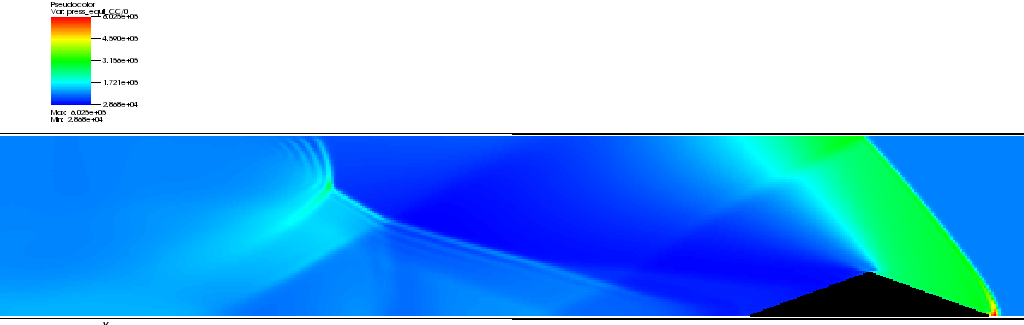
\includegraphics[scale=.4]{M2wedge.png}

  \caption{$20^o$ wedge moving at Mach 2.0 through initially stationary
air.  Contour plot depicts pressure.}
  \label{figwedge}
\end{figure}
\newpage
%
%__________________________________
\subsection*{\center Cylinder in a Crossflow}
\addcontentsline{toc}{subsection}{Cylinder in a Crossflow}
\subsubsection*{\underline{Problem Description}}
In this example the domain is initially filled with air moving at a uniform velocity of $0.03m/s$  A ridgid cylinder $O.D. = 0.02m$ is placed $0.1m$ from the inlet and a passive scalar is injected into the domain through a $0.002m$ hole on in the inlet boundary of the domain.  A velocity perturbation is placed upstream of the cylinder to produce an instablity that will help trigger the onset of the K\'arm\'an vortex street.
%
\subsection*{\underline{Simulation Specifics}}
\begin{description}
\item [Component used:] \hfill rmpmice (Rigid MPM-ICE)
\item [Input file name:] \hfill \TT{cylinderCrossFlow.ups}
\item [Command used to run input file:]\hfill \\
\TT{mpirun -np 6  sus inputs/UintahRelease/MPMICE/cylinderCrossFlow.ups}

\item [Simulation Domain:]\hfill    0.3 x 0.15 x 0.001 m

\item [Cell Spacing:]\hfill \\
.00015 x .001 x .001 m (Level 0)

\item [Example Runtimes:] \hfill \\
 7ish hrs   (6 processor, 3.16 GHz Xeon)\\

\item [Physical time simulated:] \hfill 60 seconds

\item [Associated visit session:] \hfill cyl\_crossFlow.session

\end{description}

\section*{\underline{Results}}

Figure~\ref{fig:cylCrossFlow} shows a snapshot of the simulation at time $t=60sec$.  The contour
plot of the passive scalar shows the K\'arm\'an vortex street behind the cylinder at $Re=700$.
\begin{figure}
  \center
  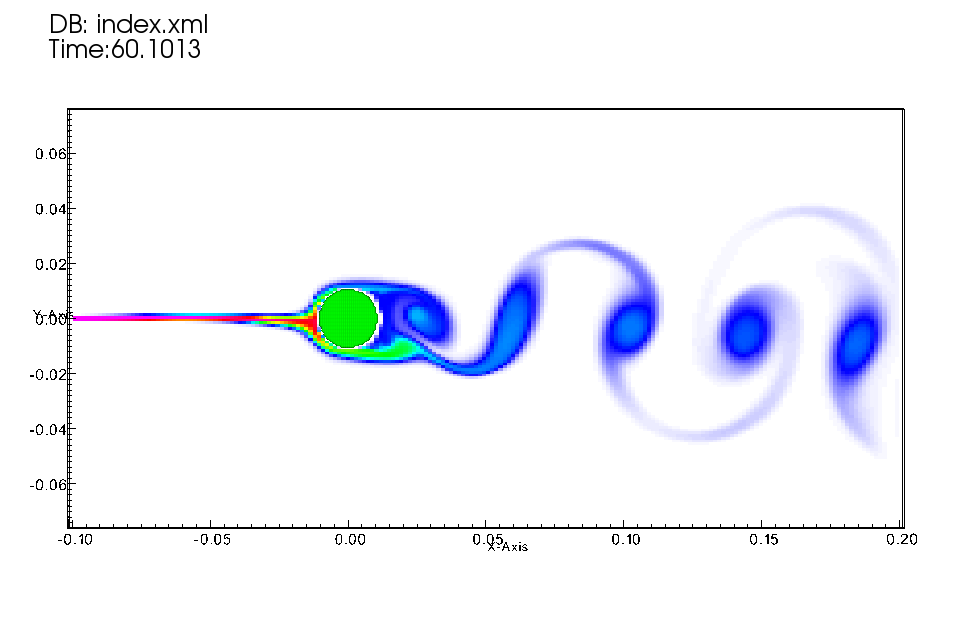
\includegraphics[scale=.5]{cylCrossFlow.png}
  \caption{Flow over a stationary cylinder, $Re=700$, a passive scalar is used as a flow marker}
  \label{fig:cylCrossFlow}
\end{figure}
%
A movie of the results is located at
\begin{Verbatim}[fontsize=\footnotesize]
  movies/cyl_crossFlow.mpg
\end{Verbatim}
\newpage

%__________________________________
\subsection*{\center Copper Clad Rate Stick (aka ``Cylinder Test")}
\addcontentsline{toc}{subsection}{"Cylinder Test"}
\subsubsection*{\underline{Problem Description}}

This is a two-dimensional version of the ``cylinder test" which is used to
characterize equations of state for explosive products.  In those tests, a
copper tube is filled with a high explosive and a detonation is initiated
at one end.  Various means are used to measure the velocity of the tube as
the high pressure product gases expand inside of it.

Here, a cylinder ($r=2.54 cm$) of QM100 is jacketed with a copper cylinder
that has a wall thickness of $0.52 cm.$   Detonation is initiated by giving
a thin layer of the explosive a high initial velocity in the axial direction
which generates a pressure that is sufficiently high to reach trigger the
detonation model.  As the detonation proceeds, the copper is pushed out of
the domain by the expanding product gases.

Note that in this example, to make run times brief, the domain is very short
in the axial direction, and is probably not sufficient for the detonation to
reach steady state.  Additionally, the domain has been reduced to two
dimensions, as symmetry is assumed in the Z-plane.  Finally, the spatial
resolution of $1.0 mm$ is a bit coarse to achieve 
convergent results.  The full three dimensional result can quickly be
obtained by commenting out the symmetry condition on the z+ plane and
uncommenting the Neumann conditions, as well as changing the spatial extents
and resolution in the Z direction to match those in the Y direction.

%
\subsubsection*{\underline{Simulation Specifics}}
\begin{description}
\item [Component used:] \hfill mpmice (MPM-ICE)
\item [Input file name:] \hfill \TT{QM100CuRS.ups}
\item [Command used to run input file:]\hfill \\
\TT{sus inputs/UintahRelease/MPMICE/QM100CuRS.ups}

\item [Simulation Domain:]\hfill    0.055 x 0.032 x 0.0005 m

\item [Cell Spacing:]\hfill \\
1.0 mm x 1.0 mm x 1.0 mm (Level 0)

\item [Example Runtimes:] \hfill \\
 20 minutes   (1 processor, 3.16 GHz Xeon)\\

\item [Physical time simulated:] \hfill 30 $\mu$seconds

\item [Associated visit session:] \hfill QM100.session

\end{description}

\subsubsection*{\underline{Results}}

Figure~\ref{fig:QM100} shows a snapshot of the simulation at time $t=60sec$.
Particles are colored by velocity magnitude, contours reflect the density of
explosive, note the highly compressed region near the shock front.
\begin{figure}
  \center
  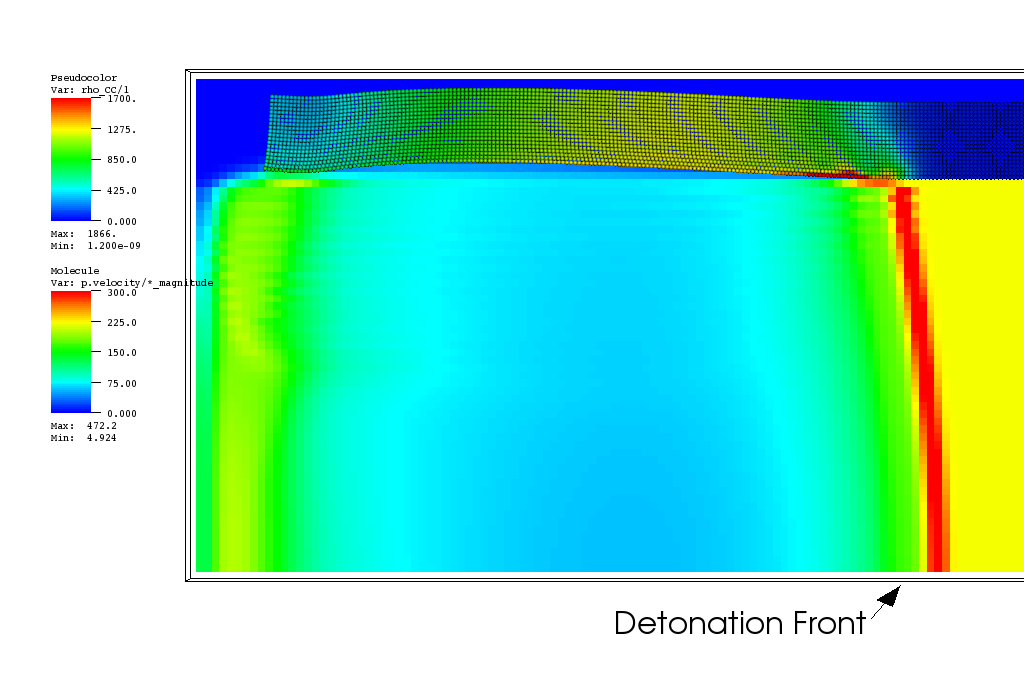
\includegraphics[scale=.45]{QM100.png}
  \caption{Detonation in a copper cylinder (2-D).  Particles are colored by
           velocity magnitude, contours indicate density of unreacted
           explosive.}
  \label{fig:QM100}
\end{figure}
%
\newpage

%________________
\section*{\center  Cylinder Pressurization Using Simple Burn}
\addcontentsline{toc}{subsection}{Cylinder Pressurization Using Simple Burn}
\subsection*{\underline{Problem Description}}
This example demonstrates use of the Simple Burn algorithm in an explosive scenario.  
The exact situation consists of a cylinder of PBX encased in steel.  For simplicity it is set up 
as a 2D simulation.  It demonstrates Symmetric boundaries as a useful construct for simplifying
the computational requirements of a problem.  The end result is the pressurization of a quarter
of a cylinder by combustion of PBX 9501.  Damage and failure models simulate cylinder failure
in a detonation scenario.  The simulation as it stands falls far short of the required physical time 
simulated for actual detonation, but demonstrates how Simple Burn can be used to pressurize 
a cylinder.  For description of Simple Burn see \ref{Sec:SimpleBurn}.

\subsection*{\underline{Simulation Specifics}}
\begin{description}
\item [Component used:] \hfill mpmice (MPM-ICE)
\item [Input file name:] \hfill guni2dRT.ups
\item [Preprocessing on input file:]\hfill \\ 1) Comment out or remove $<$max\_Timesteps$>$ on line 21 \\
2) Comment out $<$outputTimestepInterval$>$ on line 96 \\ 
3) add $<$outputInterval$>$5e-5$<$outputInterval$>$ on line 97 \\
\item [Command used to run input file:]\hfill mpirun -np 4 sus inputs/UintahRelease/MPMICE/guni2dRT.ups

\item [Simulation Domain:]\hfill    8.636 x 8.636 x 0.16933 cm

\item [Example Runtimes:] \hfill \\
2 minutes   (1 processor, 2.8 GHz Xeon)\\

\item [Physical time simulated:] \hfill 8 microseconds \\ 


\item [Associated visit session:] \hfill SimpleBurn.session

\end{description}

\newpage

\section*{\underline{Results}}
With the recession of mass comes a pressure increase that causes the
case to expand outward.  A snapshot of pressure after the 0.4
milliseconds can be seen in Figure~\ref{figsimburn1}.  At this time
pressure has increased to three-fold its initial value.  A later
snapshot Figure~\ref{figsimburn2} shows the response of the steel
cylinder to increased pressure.  Note that mass flux will scale
according to \ref{simburneqn}.  Another interesting view of the
simulation can be seen in Figure~\ref{figsimburn3}.  On the left is
the normal particle and pseudocolor map representing solid mass and
pressure respectively.  On the top right, change in pressure during
the timestep can be seen (delP\_Dilatate).  The bottom shows change in
pressure due to mass exchange (del\_MassX).  See table
\ref{table:iceLabels} for description of these variables.


% \begin{figure}
%   \center
%   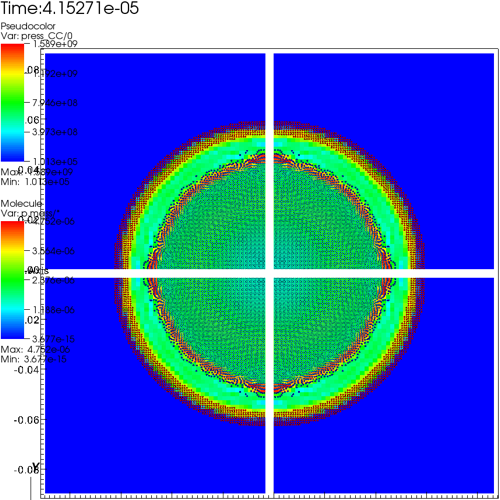
\includegraphics[scale=.3]{SimpleBurn0000.png}

%   \caption{Receding PBX9501 leads to pressure increase in cylindrical steel shell.}
%   \label{figsimburn1}
% \end{figure}

% \begin{figure}
%   \center
%   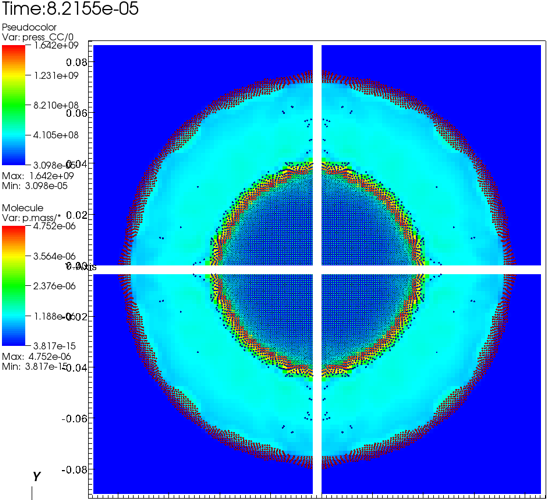
\includegraphics[scale=.3]{SimpleBurn0001.png}

%   \caption{Pressure increase causes cylinder to respond.}
%   \label{figsimburn2}
% \end{figure}

% \begin{figure}
%   \center
%   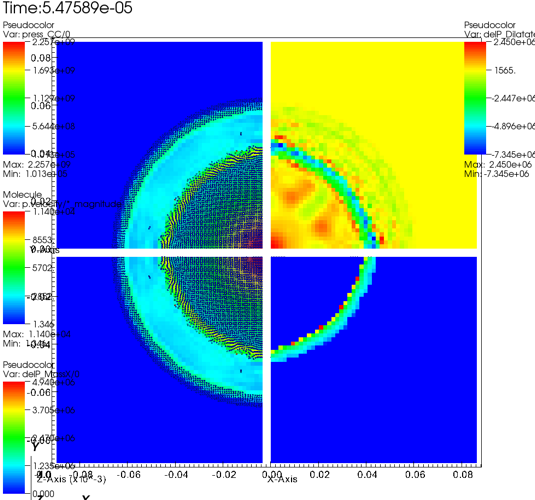
\includegraphics[scale=.3]{SimpleBurn0002.png}

%   \caption{The left half of the image represents particles as spheres colored according to mass and pressure as background color.  Top-right shows delP\_Dilatate and bottom-right shows delP\_MassX.}
%   \label{figsimburn3}
% \end{figure}


\begin{figure}
  \centering
  \vspace{-60pt}
  \subfloat[Receding PBX9501 leads to pressure increase in cylindrical steel shell]{\label{figsimburn1}
    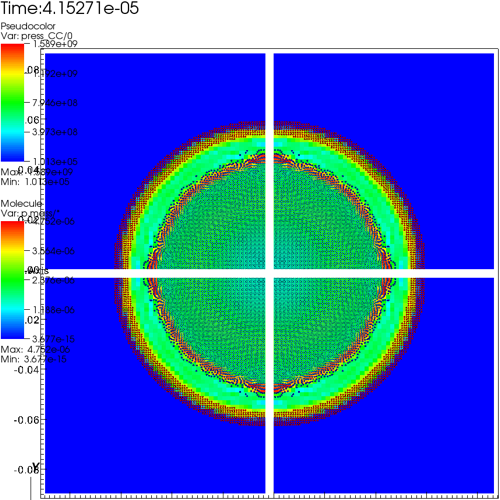
\includegraphics[width=.4\textwidth]{SimpleBurn0000.png}}
  \hspace{10pt}
  \subfloat[Pressure increase causes cylinder to respond]{\label{figsimburn2}
    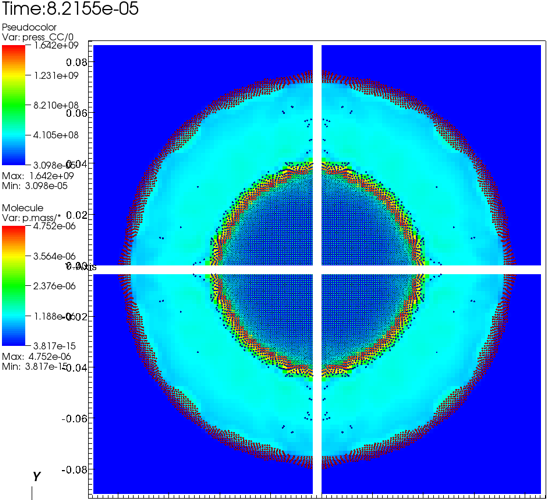
\includegraphics[width=.4\textwidth]{SimpleBurn0001.png}}
  \hspace{10pt}
  \subfloat[The left half of the image represents particles as spheres colored according to mass and pressure as background color.  Top-right shows delP\_Dilatate and bottom-right shows delP\_MassX]{\label{figsimburn3}
    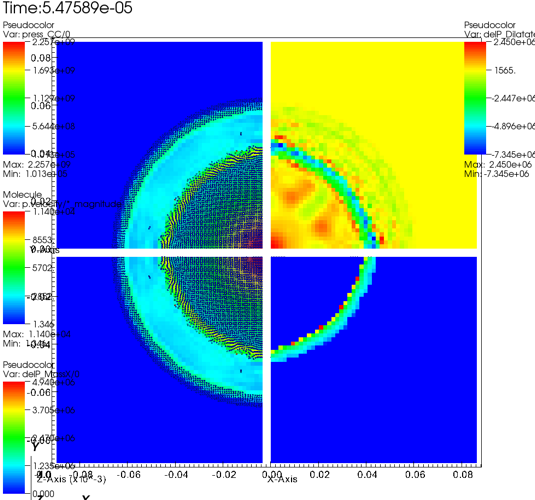
\includegraphics[width=.4\textwidth]{SimpleBurn0002.png}}
  \caption{}
  \label{}
  \vspace{-20pt}
\end{figure}


\newpage


%
\section*{\center Exploding Cylinder Using Steady Burn}
\addcontentsline{toc}{subsection}{Exploding Cylinder Using Steady Burn}
\subsection*{\underline{Problem Description}}
This problem consistes of a cylinder initially at 600 K causing burning.  Steady Burn acts as the model for burning of HE material.  More information on Steady Burn can be found in \ref{Sec:SteadyBurn}.  The cylinder is build from an outer shell of steel covering a hollow bored cylinder of PBX9501.  The simulation demonstrates the violence of explosions when large voids allow rapid expansion of surface area due to collapse of explosive material into the bore.  Information on the violence of explosions with solid and hollow cores can be attained in \cite{ref:wighteddings}.  

\subsection*{\underline{Simulation Specifics}}
\begin{description}
\item [Component used:] \hfill mpmice (MPM-ICE)
\item [Input file name:] \hfill SteadyBurn\_2dRT.ups
\item [Preprocessing on input file:]\hfill \\ 1) Comment out or remove $<$max\_Timesteps$>$ \\ 2) Comment out $<$outputTimestepInterval$>$ and uncomment $<$outputInterval$>$ around line 101 \\
\item [Command used to run input file:]\hfill mpirun -np 4 sus inputs/UintahRelease/MPMICE/SteadyBurn\_2dRT.ups

\item [Simulation Domain:]\hfill    9 x 9 x 0.1 cm

\item [Example Runtimes:] \hfill \\
 5 hours   (1 processor, 2.8 GHz Xeon)

\item [Physical time simulated:] \hfill 3 milliseconds \\ 


\item [Associated visit session:] \hfill SteadyBurn.session

\end{description}

\newpage

\section*{\underline{Results}}

Figure~\ref{figsteadyburn1} shows a nice view of the cylinder as the
PBX particles within is collapsing into the void, creating more
burnable surface area resulting in more violent explosion.  Figure
~\ref{figsteadyburn2} shows a view of the cylinder as the steel
container begins to expand outward.  Arrows represent the speed at
which the particles in the steel case are expanding outward.
Figure~\ref{figsteadyburn3} shows cell flagged as burning by Steady
Burn.

% \begin{figure}
%   \center
%   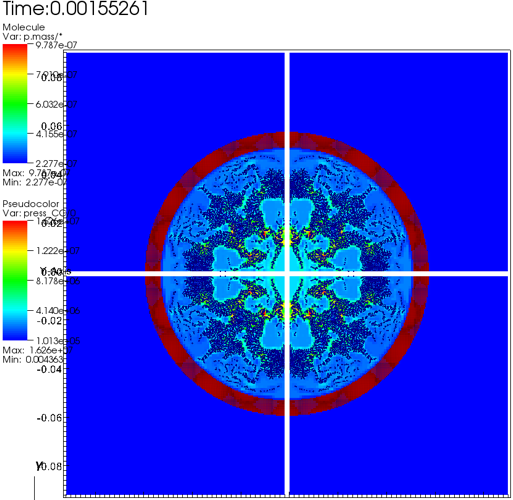
\includegraphics[scale=.3]{SteadyBurn0000.png}

%   \caption{Collapse of PBX into hollow bore of explosive device.}
%   \label{figsteadyburn1}
% \end{figure}

% \begin{figure}
%   \center
%   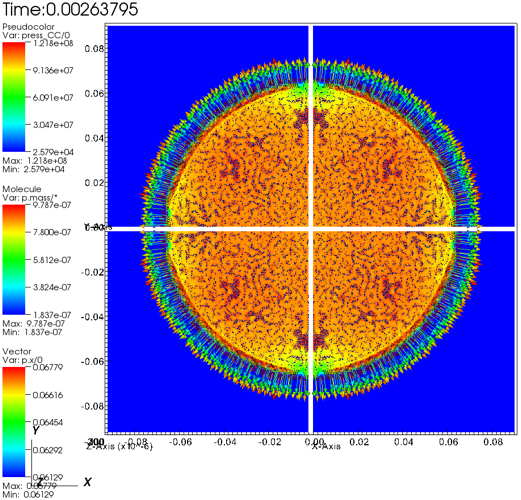
\includegraphics[scale=.4]{SteadyBurn0001.png}

%   \caption{Expansion of steel casing as explosion occurs--response to pressure build-up.}
%   \label{figsteadyburn2}
% \end{figure}

% \begin{figure}
%   \center
%   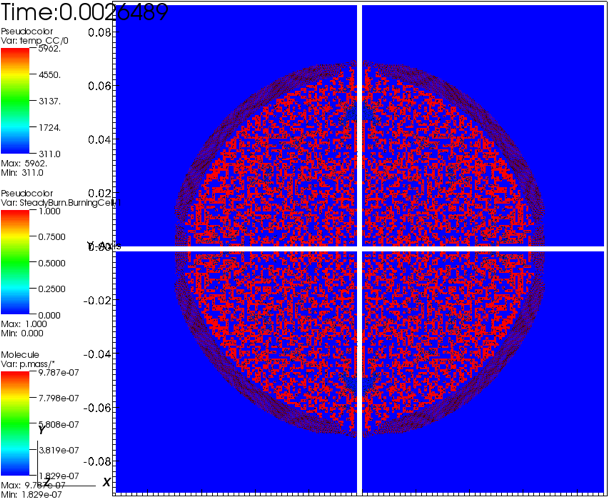
\includegraphics[scale=.4]{SteadyBurn0002.png}

%   \caption{Burning Cells denoted by red squares.}
%   \label{figsteadyburn3}
% \end{figure}


\begin{figure}
  \centering
  \vspace{-40pt}
  \subfloat[Collapse of PBX into hollow bore of explosive device]{\label{figsteadyburn1}
    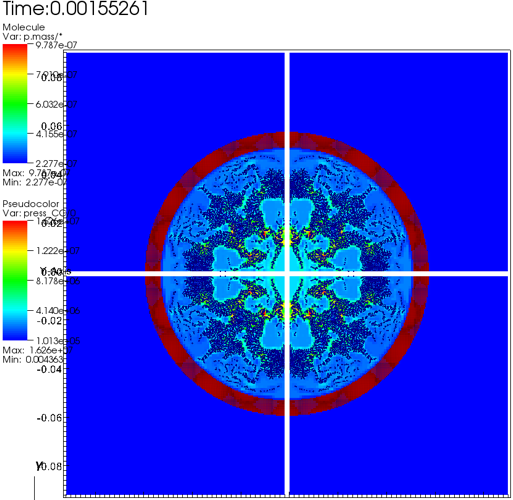
\includegraphics[width=.4\textwidth]{SteadyBurn0000.png}}
  \hspace{10pt}
  \subfloat[Expansion of steel casing as explosion occurs--response to pressure build-up]{\label{figsteadyburn2}
    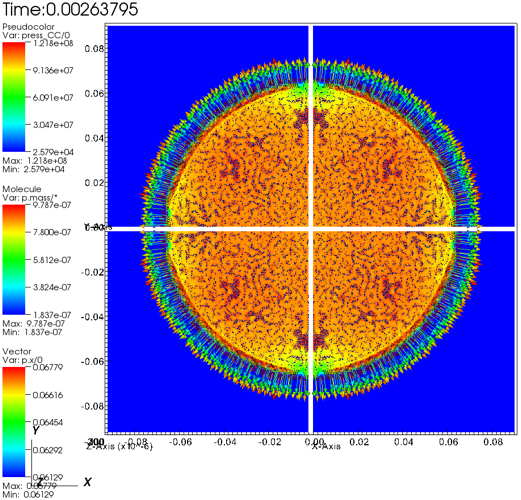
\includegraphics[width=.4\textwidth]{SteadyBurn0001.png}}
  \hspace{10pt}
  
  \subfloat[Burning Cells denoted by red squares]{\label{figsteadyburn3}
    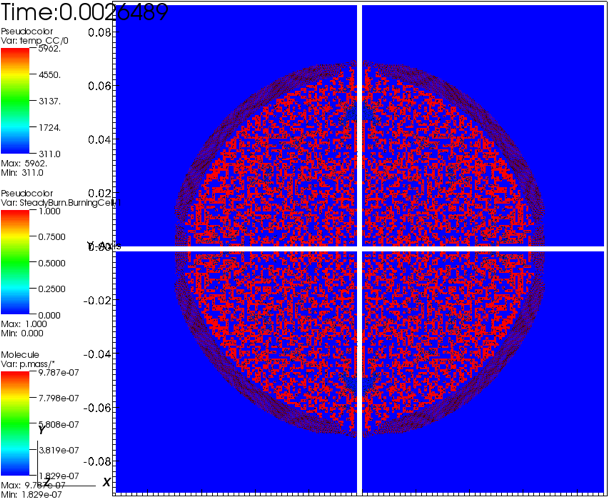
\includegraphics[width=.4\textwidth]{SteadyBurn0002.png}}
  \caption{}
  \label{}
  

\end{figure}


\newpage
%
\newpage
\section*{\center  T-Burner Example Using Unsteady Burn}
\addcontentsline{toc}{subsection}{T-Burner Example Using Unsteady Burn}
\subsection*{\underline{Problem Description}}
The T-Burner problem was inspired by  an article by Jerry Finlinson, Richard Stalnaker and Fred Blomshield in which a T-Burner apparatus was pressurized to a given pressure and ignited \cite{ref:finlinson1}.  The T-Burner composed of a cylinder with HMX on each circular ends, and a pressure inlet halfway between the HMX caps pumps pressure into the vessel parallel to those walls.  Finlinson, et. al. measured pressure oscillations in the chamber and this simulation mimics the behavior found of Finlinson's 500 psi experiment.  For simplicity and resource minimization, the simulation is set up as a 2D T-Burner.  The graphs below shows the pressure oscillations over time compared with that from \cite{ref:finlinson1}.  This simulation demonstrates the utility of Unsteady Burn in simulations where pressure oscillations occur in small places.  For more information on Unsteady Burn see \ref{Sec:UnsteadyBurn}.

\subsection*{\underline{Simulation Specifics}}
\begin{description}
\item [Component used:] \hfill mpmice (MPM-ICE)
\item [Input file name:] \hfill \TT{TBurner\_2dRT.ups}
\item [Command used to run input file:]\hfill mpirun -np 4 sus TBurner\_2dRT.ups

\item [Simulation Domain:]\hfill    0.822 x 0.138 x 0.003 m

\item [Example Runtimes:] \hfill \\
 25 minutes   (1 processor, 2.8 GHz Xeon)\\

\item [Physical time simulated:] \hfill 0.46 milliseconds \\ 
0.46 milliseconds of simulation equates flag $<$max\_Timesteps$>$410$</$max\_Timesteps$>$ \\ \\
Notes: \\
1)Remove line from input file to allow simulation to run full 0.25 seconds \\
2)Comment out $<$outputTimestepInterval$>$ and uncomment $<$outputInterval$>$ to make output $\Delta t$ constant \\ 

\item [Associated visit session:] \hfill TBurner.session

\end{description}

\newpage

\section*{\underline{Results}}

Figure~\ref{figtburn1}, ~\ref{figtburn2} and ~\ref{figtburn3} show successive snapshots of the simulation.  Contour plot depicts pressure and represents the wave front as it oscillates between two sheets of burning PBX 9501.  Figure ~\ref{figtburnVel} shows velocities of gas cells.
% \begin{figure}
%   \center
%   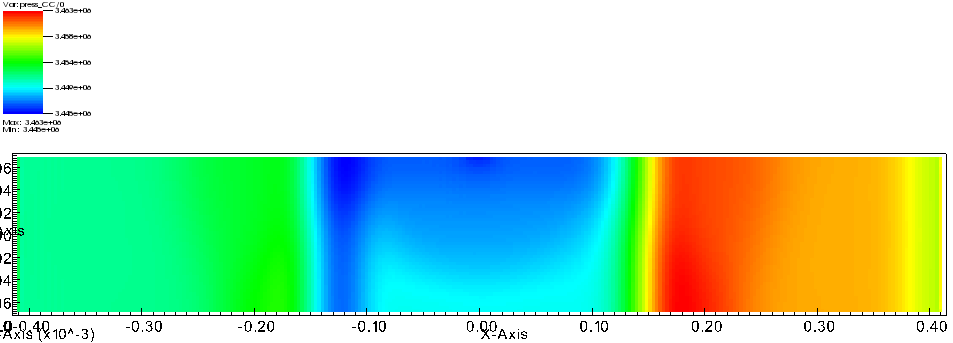
\includegraphics[scale=.4]{TBurner0000.png}

%   \caption{Time 1: Oscillatory behavior in the form of a pressure wave in a T-Burner.  Contour plot depicts pressure.}
%   \label{figtburn1}
% \end{figure}

% \begin{figure}
%   \center
%   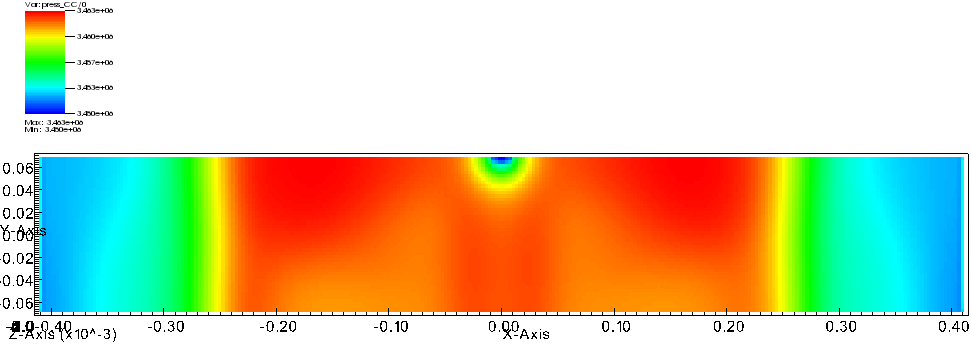
\includegraphics[scale=.4]{TBurner0001.png}

%   \caption{Time 2: Oscillatory behavior in the form of a pressure wave in a T-Burner.  Contour plot depicts pressure.}
%   \label{figtburn2}
% \end{figure}
% \begin{figure}
%   \center
%   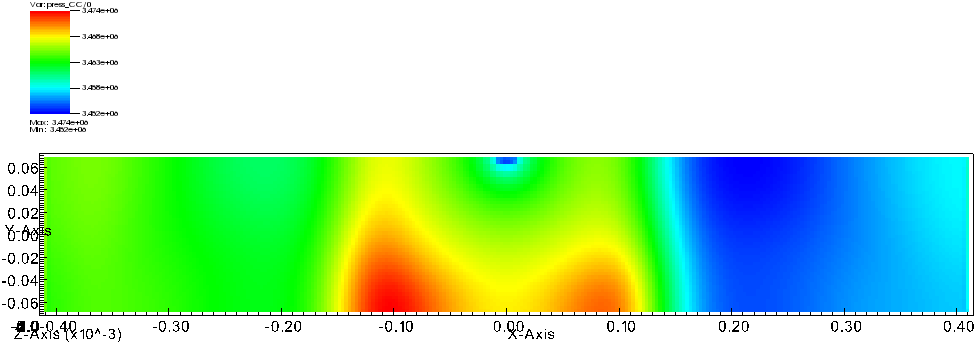
\includegraphics[scale=.4]{TBurner0002.png}

%   \caption{Time 3: Oscillatory behavior in the form of a pressure wave in a T-Burner.  Contour plot depicts pressure.}
%   \label{figtburn3}
% \end{figure}


\begin{figure}[H]
  \centering
  \vspace{-80pt}
  \subfloat[Time 1: Oscillatory behavior in the form of a pressure wave in a T-Burner.  Contour plot depicts pressure]{\label{figtburn1}
  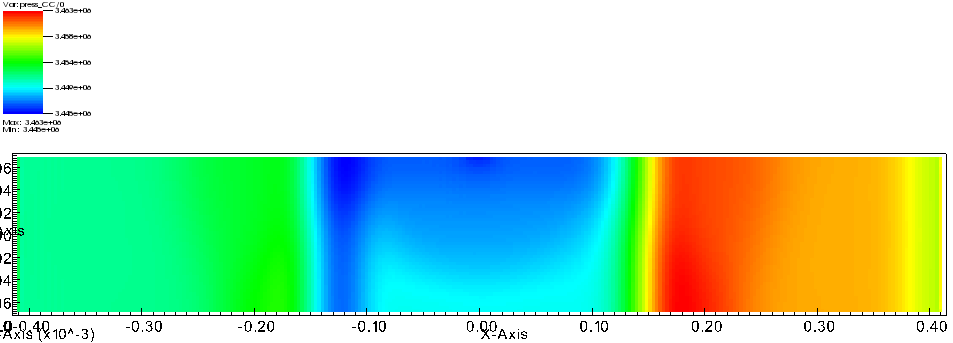
\includegraphics[scale=.4]{TBurner0000.png}}

   \subfloat[Time 2: Oscillatory behavior in the form of a pressure wave in a T-Burner.  Contour plot depicts pressure]{\label{figtburn2}
     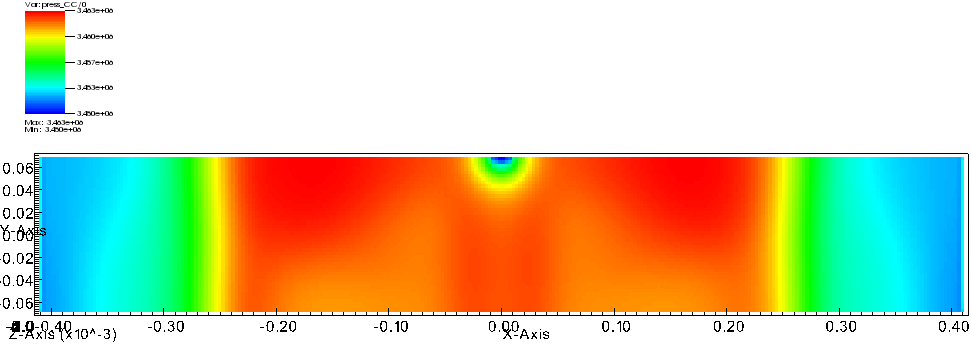
\includegraphics[scale=.4]{TBurner0001.png}}

   \subfloat[Time 3: Oscillatory behavior in the form of a pressure wave in a T-Burner.  Contour plot depicts pressure]{\label{figtburn3}
     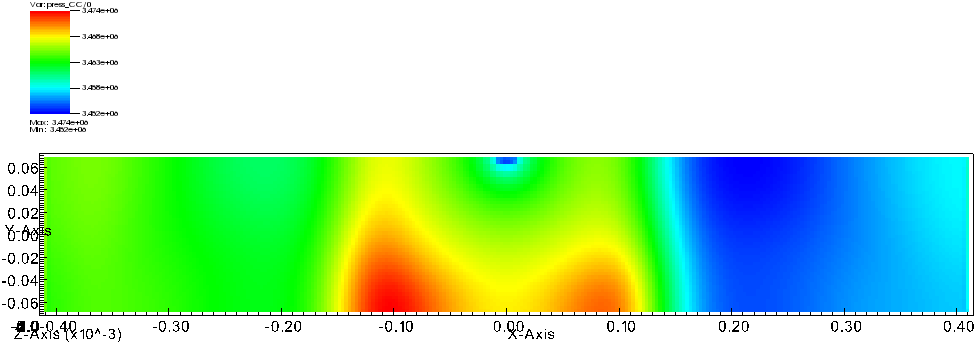
\includegraphics[scale=.4]{TBurner0002.png}}

   \subfloat[Velocity vectors of cell material.  Shows how the pressure causes gas to move]{\label{figtburnVel}
  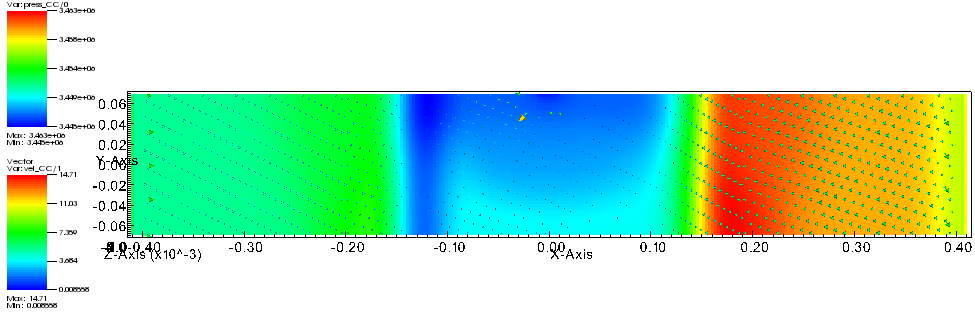
\includegraphics[scale=.4]{TBurnerVel0000.png}}

  \caption{}
  \label{}
  \vspace{-30pt}
\end{figure}


Figure~\ref{figtburnVel} shows a snapshot of the simulation at the same instant as the 
previous figure.  The contour plot depicts pressure.  The arrows are vectors depicting
the importance   
% \begin{figure}
%   \center
%   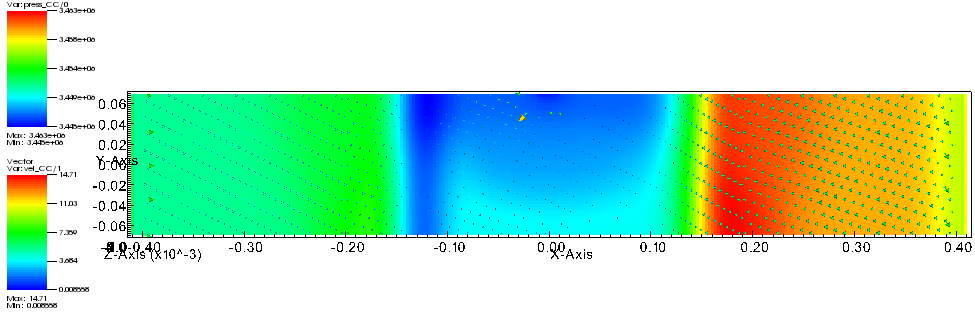
\includegraphics[scale=.4]{TBurnerVel0000.png}

%   \caption{Velocity vectors of cell material.  Shows how the pressure causes gas to move.}
%   \label{figtburnVel}
% \end{figure}

%
%__________________________________
\newpage
\section*{\center  Pinwheel}
\addcontentsline{toc}{subsection}{Pinwheel}
\subsection*{\underline{Problem Description}}
This simulation provides an example of fluid-solid interaction through driving a pinwheel via a supersonic jet of air. A 500 m/s jet of air is directed at the face of one of four fins attached to a hollowed cylinder surrounding a pin. This continuous jet of air spins the wheel around the stationary pin creating an easily visually verifiable fluid-solid interaction model. 

\subsection*{\underline{Simulation Specifics}}
\begin{description}
\item [Component used:] \hfill mpmice (MPM-ICE)
\item [Input file name:] \hfill \TT{pinWheel.ups}
\item [Command used to run input file:]\hfill 
mpirun -np 6 sus inputs/UintahRelease/MPMICE/pinWheel.ups

\item [Simulation Domain:]\hfill    4.5 x 3.0 x 4.5 m

\item [Example Runtimes:] \hfill \\
 10 hours   (6 processors, 2.66 GHz Xeon)\\

\item [Physical time simulated:] \hfill 1 second \\ 

\item [Associated visit session:] \hfill pinWheel.session

\end{description}

\newpage

\section*{\underline{Results}}


\begin{figure}
  \centering
  \vspace{-40pt}
  \subfloat[Pinwheel driven by a jet of air]{\label{pinwheel1}
    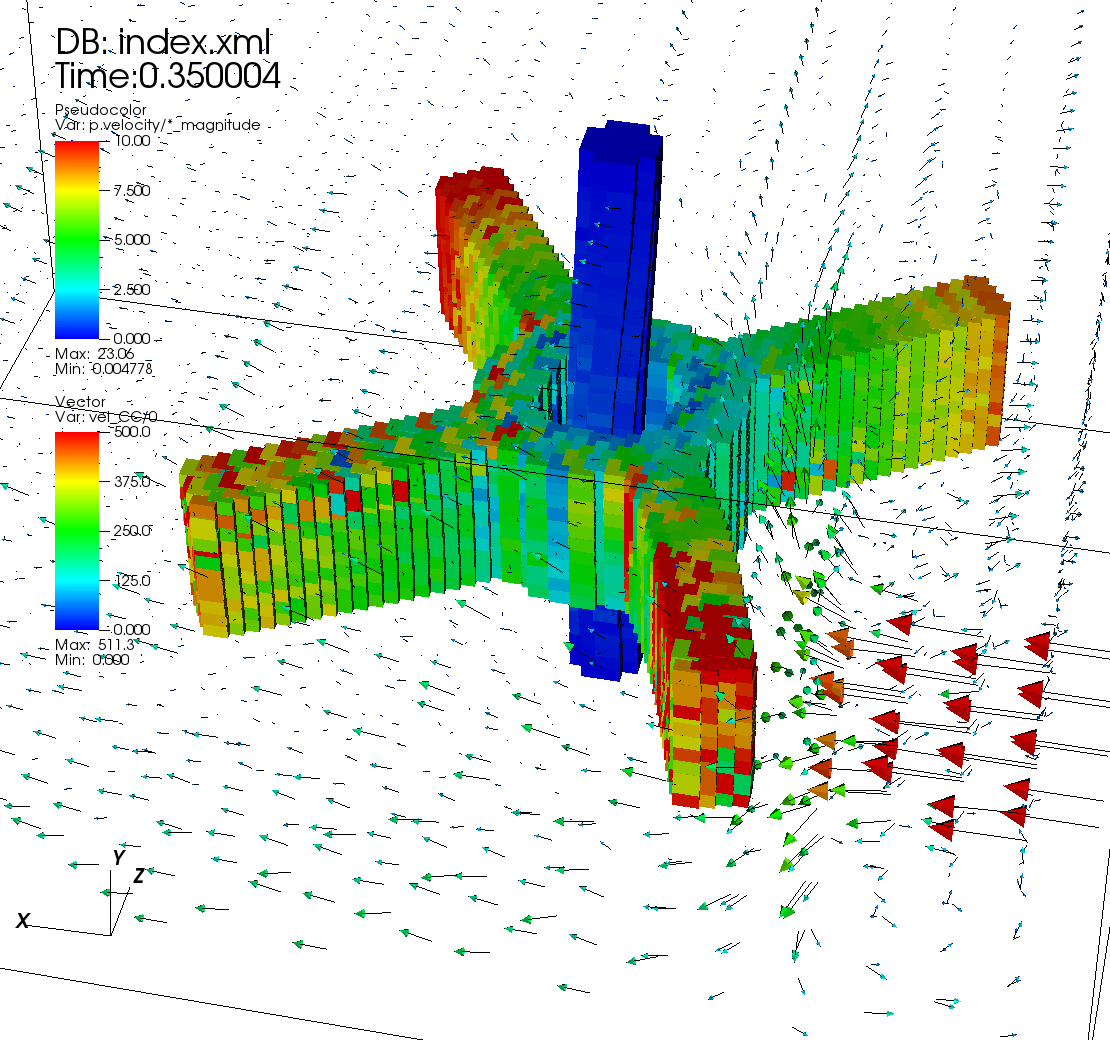
\includegraphics[width=.8\textwidth]{pinWheel.png}}
  \hspace{10pt}
  \caption{}
  \label{}

\end{figure}

Figure~\ref{pinwheel1} shows a visualization of the pinwheel alongside the air jet represented by the velocity vectors. The air jet contacts a fin on the wheel causing it to continuously rotate counterclockwise as seen by the colored velocity of the boxes.  

\bibliographystyle{plain}
\bibliography{ice}
